\documentclass[12pt,preprint]{aastex}
\usepackage{amsmath}
\usepackage[]{graphicx, epstopdf}
\usepackage{indentfirst}
\usepackage{lscape}
\usepackage{afterpage}
\usepackage{rotating}
\let\captionbox\undefined
%\usepackage{caption}
\usepackage[font=footnotesize,labelfont={footnotesize,bf}]{caption}

%\captionsetup{width=6.3in,font=footnotesize}
\usepackage{wrapfig}
\usepackage{multicol}
\usepackage{textcomp}
\newcommand{\textapprox}{\raisebox{0.5ex}{\texttildelow}}

\usepackage{tabu}
\usepackage{multirow}

\usepackage{xcolor}
\usepackage{ulem}

\usepackage[compact]{titlesec}
\titleformat{\section}{\normalsize\bfseries\centering}{\thesection}{1em}{}
\titleformat{\subsection}[runin]{\normalsize\bfseries}{\thesubsection}{0.5em}{}[:$\:\:\:$]
\titleformat{\subsubsection}[runin]{\normalsize\bfseries}{\thesubsubsection}{0.5em}{}[:$\:\:\:$]
\titlespacing{\section}{2pt}{*0}{*0}
\titlespacing{\subsection}{0pt}{2pt}{0pt}
\titlespacing{\subsubsection}{0pt}{2pt}{0pt}

\setlength{\textwidth}{6.5in}
\setlength{\hoffset}{0in}
\setlength{\oddsidemargin}{0in}
\setlength{\evensidemargin}{0in}

\setlength{\textheight}{8.75in}
\setlength{\voffset}{0in}
\setlength{\topmargin}{0in}
\setlength{\headsep}{0.25in}
\setlength{\headheight}{0in}


%Some handy-dandy commands
%***Distance and Length***
\newcommand{\meters}{\mbox{m}}
\newcommand{\cm}{\mbox{cm}}
\newcommand{\km}{\mbox{km}}
\newcommand{\dpc}{d_{pc}}
\newcommand{\au}{\mbox{AU}}
\newcommand{\microns}{\mu\mbox{m}}
\newcommand{\rsun}{R_{\sun}}
\newcommand{\rjup}{R_J}
\newcommand{\rearth}{R_{\earth}}

%***Times***
\newcommand{\hours}{\mbox{ hrs}}
\newcommand{\seconds}{\mbox{ s}}
\newcommand{\years}{\mbox{ yrs}}

%**Mass**
\newcommand{\kg}{\mbox{kg}}
\newcommand{\msun}{M_{\sun}}
\newcommand{\mearth}{M_{\earth}}
\newcommand{\mjup}{M_J}






% Alter some LaTeX defaults for better treatment of figures:
    % See p.105 of "TeX Unbound" for suggested values.
    % See pp. 199-200 of Lamport's "LaTeX" book for details.
    %   General parameters, for ALL pages:
    \renewcommand{\topfraction}{0.9}    % max fraction of floats at top
    \renewcommand{\bottomfraction}{0.8} % max fraction of floats at bottom
    %   Parameters for TEXT pages (not float pages):
    \setcounter{topnumber}{2}
    \setcounter{bottomnumber}{2}
    \setcounter{totalnumber}{4}     % 2 may work better
    \setcounter{dbltopnumber}{2}    % for 2-column pages
    \renewcommand{\dbltopfraction}{0.9} % fit big float above 2-col. text
    \renewcommand{\textfraction}{0.07}  % allow minimal text w. figs
    %   Parameters for FLOAT pages (not text pages):
    \renewcommand{\floatpagefraction}{0.7}      % require fuller float pages
        % N.B.: floatpagefraction MUST be less than topfraction !!
    \renewcommand{\dblfloatpagefraction}{0.7}   % require fuller float pages

%%%%%%%%%%%%%%%%%%%%%%%%%%%%%%%%%%%%%%%%%%%%%%%%%%%%%%%%%%%%%%%%%%%%%%%%%%%%%%%%
%%
%% The following section outlines numerous optional output that
%% can be displayed in the front matter or as running meta-data.
%%
%% If you wish, you may supply running head information, although
%% this information may be modified by the editorial offices.
\shorttitle{Sample article}
\shortauthors{Schwarz et al.}
%%
%% You can add a light gray and diagonal water-mark to the first page 
%% with this command:
% \watermark{text}
%% where "text", e.g. DRAFT, is the text to appear.  If the text is 
%% long you can control the water-mark size with:
%  \setwatermarkfontsize{dimension}
%% where dimension is any recognized LaTeX dimension, e.g. pt, in, etc.
%%
%%%%%%%%%%%%%%%%%%%%%%%%%%%%%%%%%%%%%%%%%%%%%%%%%%%%%%%%%%%%%%%%%%%%%%%%%%%%%%%%

%% This is the end of the preamble.  Indicate the beginning of the
%% manuscript itself with \begin{document}.

\begin{document}

%*****************
% cover page
%****************
\thispagestyle{empty}

\raggedright
\huge
Astro2020 APC White Paper \linebreak

GMagAO-X: extreme adaptive optics \& coronagraphy for GMT at first light \linebreak
\normalsize

\noindent \textbf{Thematic Areas:} \linebreak
\hspace*{60pt} $\square$ Planetary Systems \linebreak
\hspace*{60pt} $\square$ Star and Planet Formation \linebreak
\hspace*{60pt}  $\square$  Stars and Stellar Evolution \linebreak
  
\textbf{Corresponding Author:}
Name: Jared R. Males \linebreak
Institution:  University of Arizona \linebreak
Email: jrmales@email.arizona.edu \linebreak
 
\textbf{Co-authors:} (names and institutions)
  \linebreak
Laird M. Close (University of Arizona) \\
Olivier Guyon (University of Arizona, Subaru Telescope)

\textbf{Abstract:} We describe plans for an ``extreme'' adaptive optics (ExAO) system for the Giant Magellan Telescope (GMT).  This instrument concept, currently called ``GMagAO-X'', is based on using existing deformable mirror (DM) and wavefront sensor (WFS) detector technology to implement a 21,000 actuator, 2000 Hz system.  Combined with state of the art coronagraphy, GMagAO-X will enable detection and characterization of exoplanets at extreme contrast ratios in groundbreaking variety.  This will include young giant planets (both from thermal emission and in the H-alpha acretion signature), older giant planets in reflected light, and temperate terrestrial planets orbiting nearby late-type stars also in reflected light.  GMagAO-X will also enable studies of circumstellar disks at unprecedented angular resolution in the visible and near-IR.  Since it is based on existing proven technology, GMagAO-X can be available at, or shortly-after, first light of the GMT, allowing the observatory to deliver groundbreaking exoplanet science almost immediately.  
\clearpage
\setcounter{page}{1}

\section{Introduction: A path to high-contrast AO imaging at/near GMT first light} \label{sec:intro}

\begin{wrapfigure}[12]{r}{3.3in}
\centering
\vspace{-0.3in}
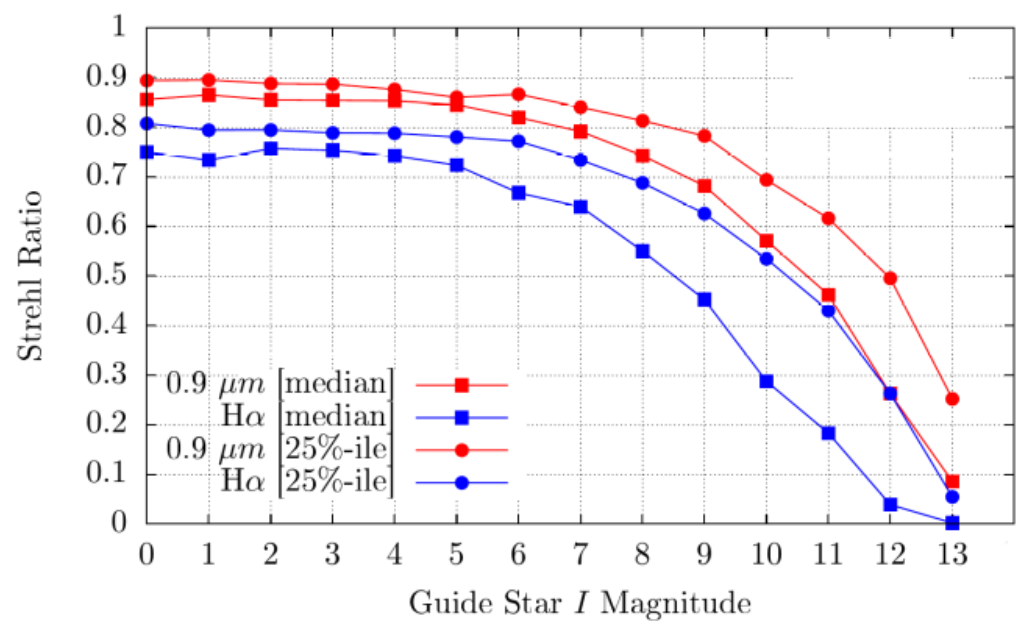
\includegraphics[width=3.1in]{figures/fig1.png}
\vspace{-0.1in}
\caption{ Strehl Ratio vs. guidestar magnitude from MagAO-X simulations \citep{2018SPIE10703E..09M}.  By maintaining the same actuator pitch, these curves can be extrapolated to the 25.4 m GMT and GMagAO-X. \label{fig:strehl} }
\end{wrapfigure}

The MagAO-X extreme adaptive optics (ExAO) system for the Magellan Clay telescope is currently under construction \citep{2018SPIE10703E..09M, 2018SPIE10703E..4YC}.  It consists of a 2040 actuator deformable mirror (DM), 3.6 kHz pyramid wavefront sensor (PyWFS), a suite of coronagraphs, and employs various post-coronagraph wavefront sensing and control (WFS\&C) techniques to optimize contrast.  MagAO-X is optimized for work in the visible, red-optical, and near-IR.  Destined for the same site as the GMT, it is an ideal testbed and demonstration system for a potential ExAO system for the GMT.

The concept we describe here, ``GMagAO-X'', is based on scaling the 2040 actuator DM from the 6.5 m Clay to the 25.4 m GMT, maintaining the same projected actuator spacing on the primary mirror.  This scaling works out to one 3000 actuator DM per 8.4 m segment.  We discuss the opto-mechanical implementation of this below.  By preserving projected actuator pitch and AO system speed, such a system will achieve the same Strehl ratio on the GMT as is projected for MagAO-X.  We show this performance in Figure \ref{fig:strehl}.

\begin{wrapfigure}[13]{r}{3.0in}
\centering
\vspace{-0.4in}
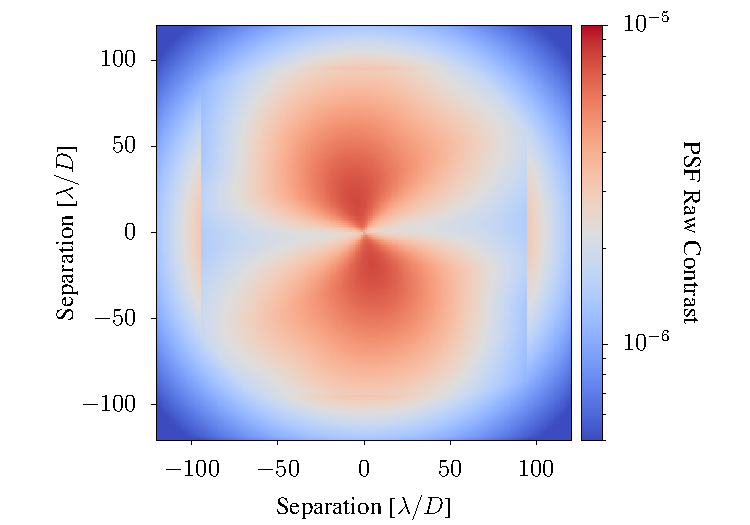
\includegraphics[width=3.1in]{figures/fig2.pdf}
\vspace{-0.25in}
\caption{ Post-coronagraph raw contrast for GMagAO-X using the semi-analytic model of Males and Guyon (2018), for an I=8 mag star such as Prox. Cen.   \label{fig:contrast} }
\end{wrapfigure}

Due to the finer sampling of atmospheric turbulence power, the larger diameter of the GMT results in a significant improvement in post-coronagraph contrast. This goes as $\propto D^2$, hence the GMT will deliver a 15x improvement over the 6.5 m Clay telescope in terms of raw contrast.  The resulting photon-noise limited exposure time improvement goes as $\propto D^4$, an improvement in by a factor of 233.  \citet{2018JATIS...4a9001M} presented a semi-analytic framework for modeling ExAO systems.  The result for an I=8th mag star, such as Proxima Centauri, is shown in Figure 2.

\section{Key Science Goals and Objectives}

Here we highlight three of the most ambitious goals for GMagAO-X.  We emphasize that an instrument optimized to conduct these science cases will be able to carry out many less demanding science programs, such as discovery and characterization of giant exoplanets \citep[Astro2020:][]{2019BAAS...51c.496B,2019BAAS...51c.505B}, the study of tight binary stars \citep[Astro2020:][]{2019BAAS...51c.483S}, high spatial and spectral resolution imaging of stellar surfaces, and the study of asteroid surfaces at high spatial resolution (to name a few).


\subsection{A GMT Survey of Temperate Exoplanets and a Search for Biosignatures on the Nearest Terrestrial Worlds}

To demonstrate the enormous scientific potential of an ExAO+Coronagraph instrument on the GMT, we analyze the existing database of known exoplanets maintained by the NASA Exoplanet Science Institute (NExScI).  For each star with a confirmed exoplanet we normalize any missing parameters, such as luminosity or I magnitude, using a main sequence table.  Most relevant planets are known from radial velocity (RV) surveys.  If no inclination is known, we use $\sin(60)$ to obtain a mass estimate.  The radii of these planets is determined using a mass-to-radius relationship which assumes terrestrial density to $4.1 M_\Earth$ ($1.6 R_\Earth$), and then uses a fit to Neptune, Uranus, Saturn, Jupiter, and the giant planet models of \citet{2007ApJ...659.1661F}.  This relationship is thus well suited to the “lightly irradiated” planets resolvable with the GMT.

Once an exoplanet’s radius is estimated, and its equilibrium temperature estimated from the host star parameters and its orbit, we can estimate its albedo.  For planets $< 1.6 R_\Earth$ we use the Earthshine spectrum of \citet{2006ApJ...644..551T} normalized to EPOXI photometry \citep{2013ApJ...765L..17C}, assuming a Lambertian phase curve. For larger planets, we use the geometric albedo grid of \citet{2010ApJ...724..189C}, which includes phase.  With the radius and geometric albedo, we calculate the mean contrast in reflected light over a planet’s observable orbit.	

Our baseline performance assumptions are that we reach a post-AO contrast of 10x worse than the frozen-flow predictive control predictions of \citet{2018JATIS...4a9001M}.  This is done on a per-guidestar basis, taking into account AO performance as a function of brightness.  The factor of 10 is intended to account for boiling and other non-frozen-flow disturbances, as well as sub-optimal as-built instrument performance. We assume an excellent coronagraph which suppresses the Airy pattern and also suppresses pinning of speckles.   We further assume that post-coronagraph and non-common-path WFS\&C is used to suppress quasi-static (long-lived) speckles to a level well below the residual atmospheric speckles.  The resulting residual noise sources are then atmospheric speckles and photon noise.  We include a semi-analytic model of residual atmospheric speckle lifetimes, and thus calculate SNR vs time for an exoplanet of a given brightness with these noise sources.
In Figure \ref{fig:planets} we show the 102 currently-known planets which could be detected in a single night (10 hrs) of telescope time each.  We estimate that a total of roughly 1 month of telescope nights will be needed for the entire survey.  This survey will sample a range of planet radii, including Earth-like and Neptune-like exoplanets.  It also spans a range of equilibrium temperatures corresponding to the inner Solar system.  Planets with these parameters have never been imaged or characterized in reflected light before.  See the Astro2020 science white paper by \citet{2019BAAS...51c.345M}.

\begin{figure}[h!]
\centering
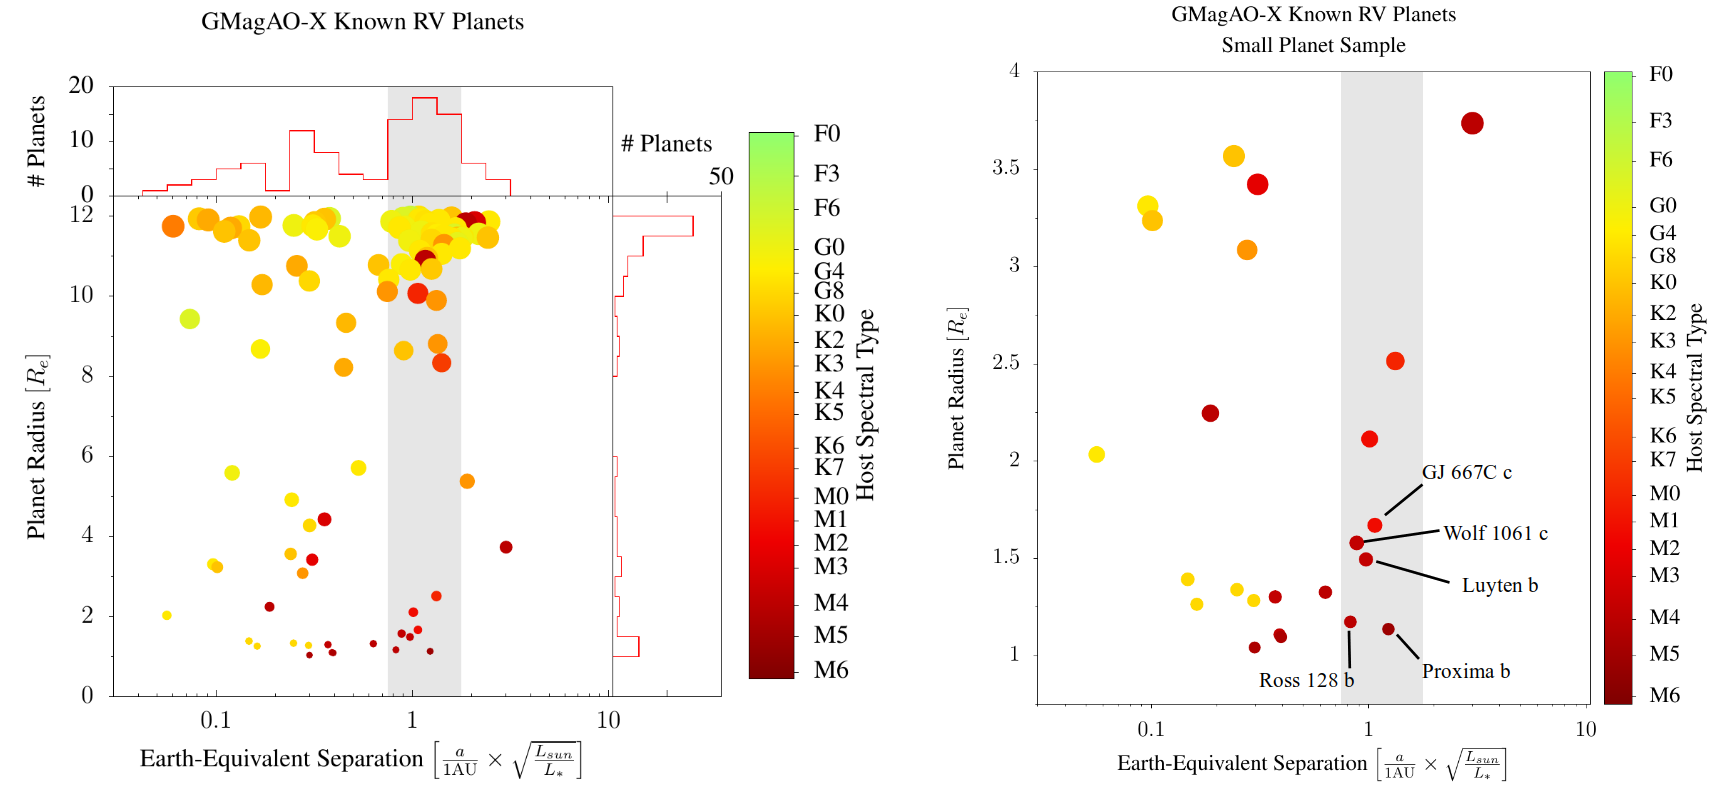
\includegraphics[width=6in]{figures/fig3.png}
\caption{GMagAO-X will enable characterization of over 100 currently known (from RV) planets.  The figure at left shows the full sample, plotted as estimated radius vs. Earth-equivalent separation (or “instellation”).  At right we highlight the small planets, and label the potentially habitable terrestrial planets. \label{fig:planets}}
\vspace{-0.3in}
\end{figure}

In the right hand panel of Figure \ref{fig:planets} we highlight the small ($< R_{Nep}$) sample.  In particular, we note the 5 terrestrial and potentially habitable planets orbiting within the “habitable zone” of their host star.  Once detected in broad-band imaging, these planets will then be characterized in detail.  Characterizing these exoplanets with GMagAO-X in refected light shortly after first-light of the GMT will allow a search for biosignatures around the nearest known temperate terrestrial worlds.
   
Next we assume that we achieve the same level of turbulence rejection, but are only able to suppress quasi-static speckles to a similar level and are hence dominated by long-lived correlated noise.  In this case, we would employ the high dispersion coronagraphy technique \citep[HDC,][]{2017ApJ...838...92M}, where template cross-correlation matching is used to detect the reflected stellar spectrum \citep{2017A&A...599A..16L}.  While less efficient than photometry for short-lived noise sources, HDC allows for root(t) improvement of SNR even in the presence of long-lived spatially correlated speckle noise.  To analyze this case, we use the BT-Settl \citep{2014IAUS..299..271A} to calculate the cross-correlation strength appropriate for a given spectral type, and then estimate the exposure time to detect each exoplanet in the NExScI database. Under this pessimistic performance case, the total number of detected planets (in 10 hrs or less each) is reduced to 63.
In Table 1, we summarize the parameters of the temperate terrestrial (potentially habitable) planets.  Once the initial detection is performed (in the integration times shown), these planets will be extensively characterized to search for biosignatures.

\begin{table}[h!]
\caption{Parameters of currently known terrestrial planets to be characterized by GMagAO-X. Exposure times are for an initial broad-band albedo measurement.\label{tab:tp}}
\vspace{-0.2in}
\centering
\begin{tabu}{lccccccc}
                &         &             &             &       &    & \multicolumn{2}{c}{ Exp. Time } \\
Planet          & Dist.   & Sep.        & Instell.    &  Rad.         & Contrast         & \multicolumn{2}{c}{ [sec] }     \\
                &  [pc]   & [mas]       & $S_{\Earth}$     &  $R_{\Earth}$        &         & Baseline   & Pessimistic \\ 
\hline
\hline
Proxima Cen b    &   1.3  &  37.6  &  1.23  &  1.14  &  1.6$\times 10 ^{-7}$  &  1092 &  2717 \\
Ross128 b       &   3.4  &  14.7   &  0.82  &  1.17  &  1.3$\times 10 ^{-7}$  &  4674  &  9388 \\
Luyten b         &   3.8   &  24.0   &  0.97  &  1.49  &  8.1$\times 10 ^{-8}$  &  3859  &  6092 \\
Wolf 1061 c     &   4.3  &  20.6   &  0.88  &  1.58  &  9.3$\times 10 ^{-8}$  &  2844  &  5650 \\
GJ 667C c        &  6.8   &  18.4   &  1.0  &  1.66  &  8.2$\times 10 ^{-8}$  &  14849  &  36157 \\
\hline
\end{tabu}
\end{table}

\subsection{ Acreting Protoplanets (H-alpha Planets)}

One of the greatest challenges to astronomy today is understanding the details of planet formation. Planet formation can be best informed by creating a complete sample of directly imaged protoplanets (separations, masses, accretion rates, etc. \citep[Astro2020 science white papers:][]{2019BAAS...51c.527S,2019BAAS...51c.475A}. But discovery of such protoplanets requires “catching them in the act of growing”. That means making a very sharp image that allows us to see the characteristic hydrogen gas accretion lines (Hydrogen alpha = $H\alpha$ = 656 nm the strongest such line accessible to adaptive optics). 

A clever optical trick (SDI) enables very high-contrast $H\alpha$ imaging by simultaneously making a $H\alpha$ image and a Continuum image on the science focal plane. Today our current SDI data reduction pipeline with MagAO's SDI camera produces very high-contrast images by first subtracting the scaled continuum image from the $H\alpha$ image to reveal $H\alpha$ protoplanets. With PCA, ADI and SDI data reduction pipelines we remove most of the contaminating starlight. In this manner, we have already made impressive detections of $H\alpha$ emitting protoplanets at 15-20AU with MagAO SDI  (\citet[HD142527 B,][]{2014ApJ...781L..30C}; \citet[LkCa 15 b,][]{2015Natur.527..342S}; and \citet[PDS 70 b,][]{2018ApJ...863L...8W}). 

Projecting to  GMagAO-X's contrasts we will be able to extend our search down to relatively low-mass planets like accreting Neptunes at just $\sim1$ AU separations \citep{2019BAAS...51c.527S}. This will allow a complete sample of southern gas protoplanets formation within $\sim200$ pc. 







\subsection{ Disks }
Disk science is critical to further our understanding of how planets and stars form \citep[see Astro2020 science whitepapers:][]{2019BAAS...51c.346J, 2019BAAS...51c.445W, 2019BAAS...51c.566D}.
It is a very challenging application of adaptive optics because
the disks are low surface brightness and extended objects exactly like the
uncorrected seeing halo. The best way to reveal disks is to have a high Strehl
system that puts little light into the region where the disk is. Secondarily,
post-processing techniques such as KLIP+PSF subtraction can be used to remove
residual PSF from even face-on disks.

There are two frontiers in circumstellar disk science, both of which will be
pushed by GMagAO-X. The first is ever more detailed imaging of disk geometry,
particularly in the 1-50 AU region analagous to the outer part of the Solar
System. Most disks sit at 50-150 pc, so reaching separations comparable to the Earth, Mars, and the giant
planet region requires imaging at 0.01-0.2". This is largely unexplored
territory. Existing systems push in to at best 0.15" (for example, the GPI
coronagraph radius is 0.15", the newest coronagraphic mode on HST, the STIS
BAR5, has an inner working angle of 0.15", and Subaru HiCIAO has reported disk
detect ions in to 0.2").  

The second frontier is the multiwavelength study of disks to derive the
chemical make-up and dynamical state.  Scattering efficiency is a strong
function of both size and composition, and measurements of disk brightness
over a large wavelength range help break the degeneracy between the two
(CITE Rodigas et al. 2015). The size distribution diagnoses the interplay of
planetesimal collisions that produce dust and radiation forces that remove
dust. We expect to see, for example, a change in the typical grain size from
large at the location of the dust birth ring to small in the outer reaches of
the disk. We also expect to see the scattering phase function (i.e. efficiency
with angle between the star, dust, and observer) change with wavelength ( CITE Stark
et al. 2014). We also might expect compositional gradients in the dust,
perhaps inside and outside of snow lines. To disentangle all of these requires
a large wavelength grasp from visible through near-infrared since scattering
depends on the ratio of the wavelength the grain size. This will harness GMagAO-X's ability to
image down to $\sim$ 0.5 microns.

\section{Technical Overview}

The Giant Magellan Telescope will be a 25.4-meter visible and infrared (0.32 - 25 $\mu$m) telescope located at Las Campanas Observatory in the Chilean Andes and is designed to provide unprecedented clarity and sensitivity for the observation of astrophysical phenomena. The optical design of GMT consists of seven 8.4-meter borosilicate honeycomb mirror segments that reflect light to seven secondary mirror segments in a doubly-segmented Gregorian configuration. The compact design and small pixelscale at the direct Gregorian focal plane requires fairly small instruments to take necessary astronomical data. Commissioning will be performed using a fast-steering secondary mirror assembly which, during science operations, can be replaced with a state-of-the-art adaptive secondary assembly comprised of fully adaptive segments. The adaptive secondary mirror provides a general-purpose AO capability to all instruments on the telescope, including ground layer, natural guide star, and laser tomography adaptive optics modes. High contrast AO instruments must provide additional wavefront control elements to achieve their science objectives.

GMT is currently being built by an international consortium of universities and research institutions with a deep history of pioneering telescope construction and design, quality instrumentation production, and revolutionary adaptive optics techniques and technology. The Founding Partners consist of Arizona State University (US), Astronomy Australia Limited (Australia), Australian National University (Australia), Carnegie Institution for Science (US), FAPESP-The S\~ao Paulo Research Foundation (Brazil), Harvard University (US), Korean Astronomy and Space Science Institute (South Korea), Smithsonian Institution (US), Texas A\&M University (US), University of Texas at Austin (US), University of Arizona (US), and the University of Chicago (US).

\begin{figure}[h!]
\centering
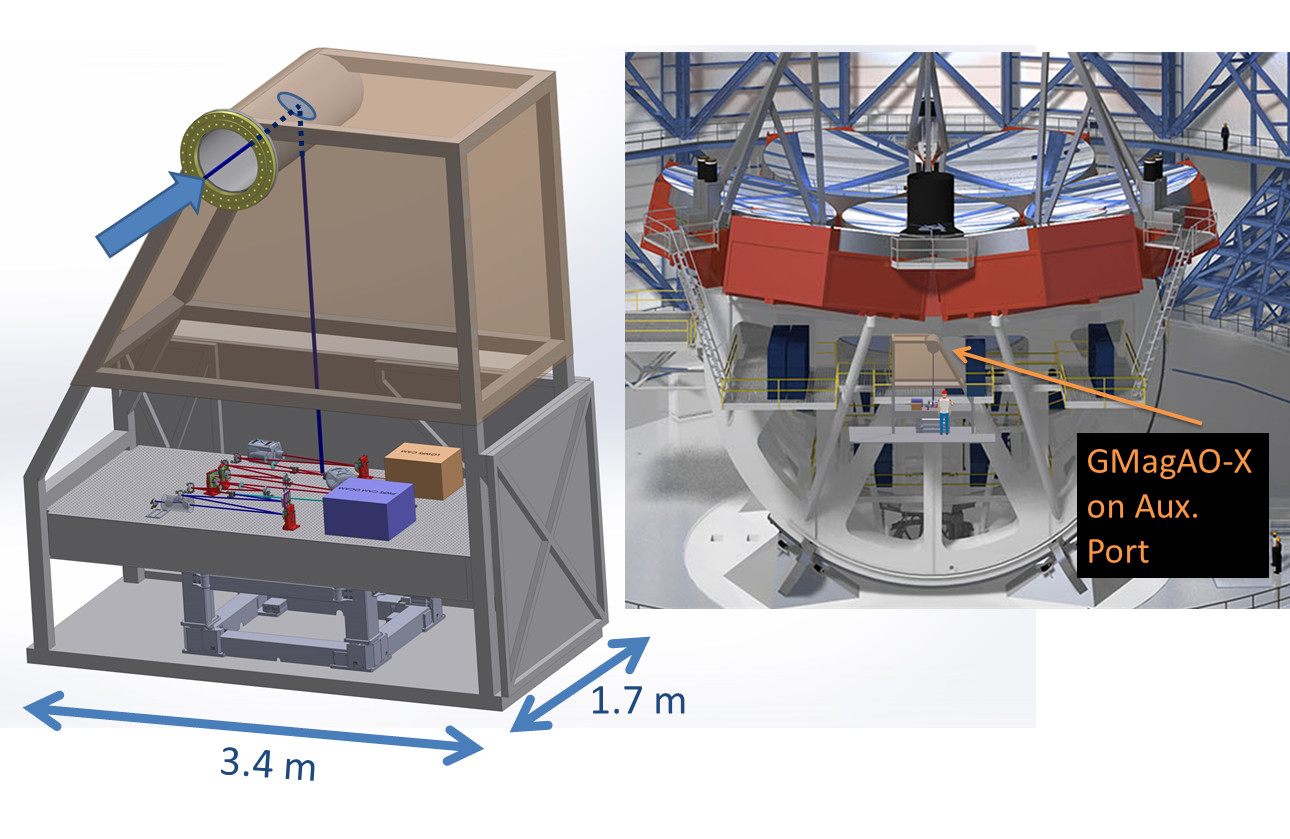
\includegraphics[width=6in]{figures/GMagAOX__fig4_no_labels_V2.png}
\vspace{-0.2in}
\caption{ GMagAO-X concept shown within the Auxiliary Port volume and mounted on the GMT elevation axis. The thick blue arrow shows the direction the light enters GMagAO-X after reflection off M3. This is a gravity invariant port which eliminates flexure and enables a vibration isolated (floating) optical 5x10' optical table. \label{fig:ap}}
\vspace{-0.1in}
\end{figure}

In Figure \ref{fig:ap} we present our notional concept of how the GMagAO-X instrument could be mounted in a gravity invariant environment at the so-called Auxilliary Port (AP). The AP is essentially equivalent to a Nasmyth port on the GMT, being on the elevation axis and so is the only place on GMT that is both gravity invariant and can also be used for imaging.  Figure \ref{fig:ap} shows how GMagAO-X will appear when mounted at the elevation axis on the GMT. As the telescope moves in elevation the instrument stays fixed w.r.t. gravity. A floating optical table (with servo control on the position of the table-- utilizing the TMC PEPSII stability system) can be employed.  This will prevent vibrations above 10Hz from coupling into the instrument (lower frequency vibrations will be removed by the AO system). 

This notional concept has established the feasibility of mounting GMagAO-X on the GMT without conflicts with already planned instruments.  The next step is to perform a complete conceptual design study to ensure that such an instrument will achieve the demanding science based requirement we motivate above, and addresses the risks unique to this instrument. 

\begin{figure} [h!]
\centering
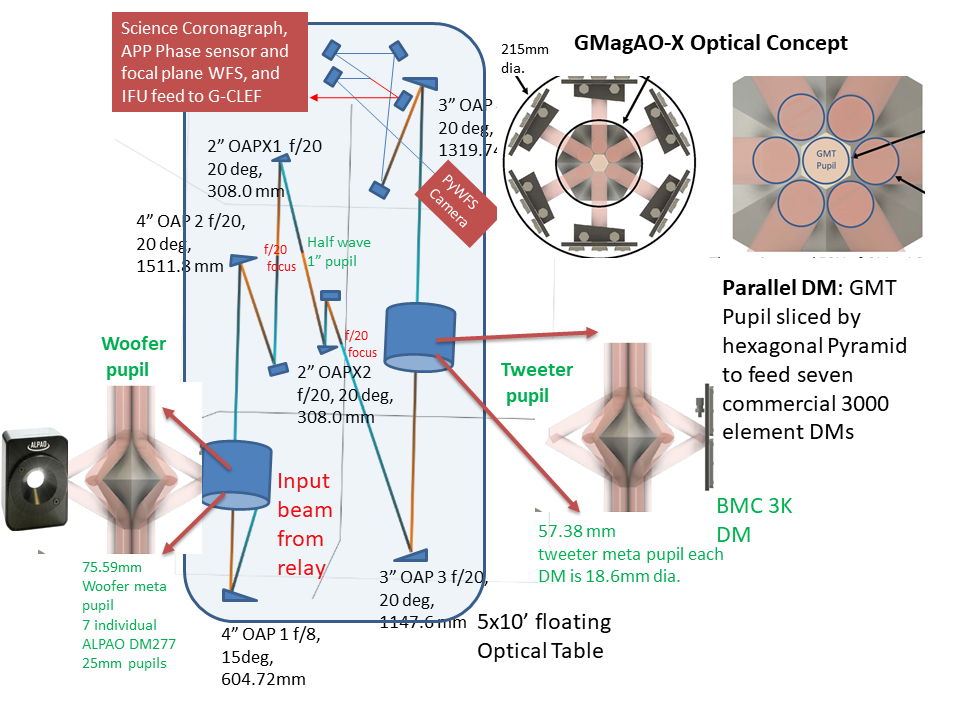
\includegraphics[width=5in]{figures/Possible_Optical_design_GMagAOX_V2.png}
\caption{ Concept for an optical design of GMagAO-X. Both the woofer and tweeter DMs take advantage of the GMT pupil with new concept called a "Parallel DM". The tweeter is 7-segment 21,000 MEMS deformable mirror using a six-sided reflective prism.  In the cartoon at left all optical paths are the same length. The center segment is passed through a central hole in the pyramid. Mechanical design renderings with different views show how such a parallel DM could be implemented in GMagAO-X's optical design on a 5x10' optical table.  \label{fig:pardm}}
\vspace{-0.1in}
\end{figure}

Achieving the $\sim$13.5 cm projected sampling of the primary mirror requires $\sim$3000 actuators per 8.4 m segment, a total of 21,000 actuators on the GMT segments.   Achieving this with a monolithic DM would require a 188x188 format device, or $\sim$35,000 actuators. The largest currently in development DM is 128x128, and no such device has yet been delivered.  While some discussion are underway for larger devices, there are no no DMs for the foreseeable future which meet our requirements. To overcome this hurdle, we have proposed a novel optical design that combines seven 3000 actuator \textit{currently available} DMs from Boston Micromachines Corp. (BMC) to work in parallel to as a combined 21,000 actuator DM. We note this "parallel DM" concept could also be applied the TMT pupil with some modifications.  This concept is illustrated in Figure \ref{fig:pardm}.

GMagAO-X will over wide wavelength coverage, extending from $\sim 0.4 \mu$m (g-band) to $\sim 2.4 \mu$m (K-band).  Focal planes will include broad-band (R$\sim$10) imagers, and fiber-fed IFUS offering spectral resolution from the R$\sim$1000 regime up to R$\sim$100,000 depending on the science case. Options include constructing new compact photonic spectrographs dedicated to GMagAO-X, and also using existing spectrographs at GMT such as G-CLEF.

\section{Technology Drivers} 

We next describe some of the key challenges and risks which must be addressed to enable ExAO on the GMT.

\textbf{The ELT ExAO-Scale DM Problem:} Achieving ~13.5 cm projected sampling of the primary mirror requires ~3000 actuators per 8.4 m segment, a total of 21,000 actuators on the GMT segments. \textbf{Risk:} Our 21,000 actuator parallel DM concept (see Fig. \ref{fig:pardm}) requires the optical disassembly/reassembly of the pupil resulting in a complicated opto-mechanical design that has not yet been demonstrated. \textbf{Mitigation Plan:} We will unambiguously prove that this parallel DM GMagAO-X design works optically and mechanically (closed-loop) with the GMT High-Contrast Phasing Testbed feeding MagAO-X in the lab as described in section \ref{subsection:testbed} below. 

\textbf{Risk:} Primary mirror segment phasing will not be achieved our $\sim$30 nm rms requirement. \textbf{Mitigation plan:} We will demonstrate phasing control is possible with the Phasing testbed described in \ref{subsection:testbed}. 

\textbf{Risk:} The pyramid wavefront sensor (PyWFS) in Fig. \ref{fig:pardm} will require $>$ 21,000 pixels per quadrant ($>$ 288 pixels across the detector) on a Pyramid WFS with $>2kHz$ frame rates and very low readnoise.  Such cameras are not currently available, though development is underway. \textbf{Mitigation Plan:}  We are already studying reflective pyramids allowing the use of 4 smaller format cameras (one for each quadrant) which already exists. These will be demonstrated in the lab as a result of ongoing research.

\textbf{Risk}: Deviations of ~10 microradians due to thermal drifts or vibrations could lead to unstable wavefront/alignment errors of the OAP optics in Fig. \ref{fig:pardm}. \textbf{Mitigation Plan:} Continue to test advanced locking kinematic optical mounts and floating optical tables as part of our phasing testbed efforts (see \ref{subsection:testbed}).

\textbf{Risk:} To eliminate high frequency non-common path vibrations we will use a floating 5x10' optical table (shown in Figs \ref{fig:ap} and \ref{fig:pardm}), yet this requires an advanced servo control of the gravity direction (to eliminate any tilts) when mounted at the GMT auxiliary port. \textbf{Mitigation Plan:} model the stability of the floating table to see if it will perform to specifications at the Aux. Port (see Fig. \ref{fig:ap}), and define the required servo system.

\textbf{Risk:} Difficult to detect biosignatures at $10^{-7}$ contrasts from the surface of the Earth (which is dominated by telluric biosignatures) \textbf{Mitigation Plan:} Use the power of High Resolution Spectroscopic Coronagraphy to exploit exoplanet Doppler shifts. Design a small ring-like "IFU" (placed at the previously determined RV angular separation of the rocky planet) with sixteen 50 micron core multi-mode fibers to feed the G-CLEF spectrograph (in a similar manner to that of G-CLEF’s Manifest feed). This should provide spectra at $R\sim218,000$ (lower resolutions possible with noiseless binning) from  $650-950$nm without crowding the sixteen traces. At such resolution the planet’s lines will shift between the fixed telluric lines and can be velocity stacked following the planet’s changing radial velocity from its orbit. In this manner biosignatures can be extracted from reflected light spectra from GMagAO-X and G-CLEF. To prove this is possible we will continue to work with the G-CLEF team to design an "exoplanet IFU". Conceptually this is planned as a sixteen sided reflective pyramid slicing the focal plane azimuthually and feeding 16 lenses bonded to $f/3$ fibers that in turn feed G-CLEF as an IFU. 

\subsection{The GMT High-Contrast Phasing Testbed}
\label{subsection:testbed}
For high contrast science cases, a pyramid wavefront sensor observing a bright on-axis guide star and controlling the ASM or a post-focal DM provides the final stage of wavefront control. While the natural guide star mode of the segmented GMT pupil has been extensively simulated, there are several areas of high risk remaining. One such area is the behavior of the pyramid wavefront sensor when atmospheric phase errors or piston vibrations across the GMT segment gaps approach half of the observing wavelength. In such conditions, the control system can occasionally “eject” segments by driving the DM in the wrong direction. Various mitigations are being considered, including more advanced control algorithms or a second focal plane sensor at a different wavelength. Another area of uncertainty is the performance of coronagraphs designed to suppress diffraction to achieve the contrast needed for exoplanet science cases. We can solve this in part by post coronagraphic focal plane wavefront sensing in combination with a classic pyramid sensor. The MagAO-X instrument follows such an architecture. 

MagAO-X is funded by the NSF MRI program and is in the late stages of development at the University of Arizona. MagAO-X provides a cost-effective foundation for the GMT High-Contrast AO Testbed. This testbed will demonstrate fine phasing control of the GMT pupil using a pyramid wavefront sensor, testing of GMT coronagraph designs and focal plane wavefront sensing techniques, and provides a pathfinder for the GMagAO-X instrument. MagAO-X will be available to the testbed at Steward Observatory for the periods when it is not in use at the 6.5m Magellan telescope. 

The testbed is a narrow-field telescope simulator that feeds the GMT pupil, with simulated atmospheric turbulence and GMT M1 segment vibration PSDs, into the MagAO-X bench (see Fig. \ref{fig:testbed}). A GMT second-channel wavefront sensor and coronagraph will also be developed, to verify our expected control strategy and contrast predictions. University of Arizona undergraduate and graduate students, under the supervision of Prof. Laird Close, will provide the majority of the labor to assemble the testbed and perform the experiments.
 
 \begin{figure} [h!]
\centering
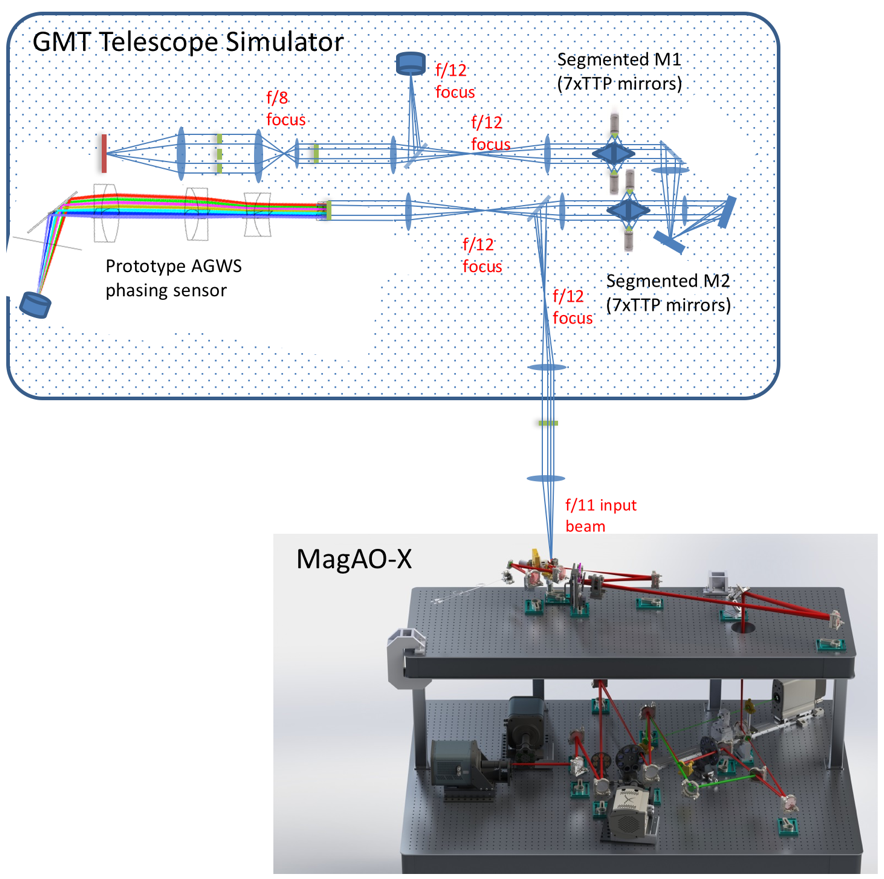
\includegraphics[width=5in]{figures/Testbed_figure.png}
\caption{GMT High-Contrast Phasing Testbed. This testbed will demonstrate rigorous closed-loop solutions to to having segment piston sensed and controlled from an initial 30 microns (not phased) down to 30 nm rms piston error while also simultaneously demonstrating closed loop AO with MagAO-X's 2040 actuator DM and Pyramid Wavefront sensor.  \label{fig:testbed}}
\end{figure}
 


\section{Organization, Partnerships, and Current Status}  
\textit{All pursuits should describe the participating
organizations, any planned partnerships, and their current status.}

\section{Schedule}
The schedule for GMagAO-X is as follows:
\vspace{-10pt}
\begin{itemize} \itemsep 0pt
\item A conceptual design study is scheduled to begin in the Fall of 2019, with Conceptual Design Review (CoDR) planned for summer 2021.  
\item The detailed design will begin immediately after CoDR.
\item Procurement of long lead-time items (e.g. DM segments) will begin in late 2021.  
\item The Preliminary Design Review will be held in early 2022.
\item A Final Deign Review will occur in late 2022.
\item Construction will begin in early 2023.
\item Shipment and deliver to the summit of Las Campanas will occur in 2025, with first-light in the 2025 to 2026 timeframe.
\item The expected instrument lifetime is at least 10 years from first-light.  
\end{itemize}

\section{Cost Estimate}

The GMagAO-X project is in the ``Medium'' ground-based instrument category (\$20M - \$70M).  An initial estimate, which includes the cost of major items such as the 7 MEMS deformable mirrors, indicates that design and construction of the ExAO system and coronagraph will be \$20M to \$30M.   



\clearpage
\thispagestyle{empty}
% References
\bibliography{references} % bibliography data in report.bib
\bibliographystyle{apj} % makes bibtex use spiebib.bst

\end{document}

% End of file `sample62.tex'.
